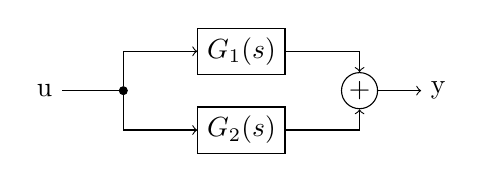
\begin{tikzpicture}
  \node (in) at (0,1) []{u};
  \node (dot) at (1,1) [draw,circle,inner sep=1,fill]{};

  \node (G1) at (2.5,1.5) [draw]{$G_1(s)$};
  \node (G2) at (2.5,0.5) [draw]{$G_2(s)$};

  \node (sum) at (4,1) [circle,draw, inner sep=1]{+};
  \node (out) at (5,1) []{y};


  \draw (in) -> (dot);
 
  \draw[->] (dot) |-  (G1);
  \draw[->] (G1) -| (sum);

  \draw[->] (dot) |-  (G2);
  \draw[->] (G2) -| (sum);

  \draw[->](sum) -- (out);

\end{tikzpicture}

